\section{Derivation of singular SDE}
\label{sec:singular_sde_app}

We consider the following SDE with additive noise; i.e., the diffusion coefficient $g$ is only a function of time.
\begin{align}
dx = f(x, t)dt + g(t)dW_t
\end{align}
The perturbation kernel $p(x_t | x_0)$ corresponding to rectified flow is Gaussian, with $p(x_t | x_0) = N(x_t; (1-t)x_0+t\mu_1, t^2\sigma_1^2I)$.
Since the perturbation kernel is Gaussian, following \citet{song2020score}, we assume that the drift term is affine; i.e. $f(x, t) \equiv f(t)x$. 
Further since $X_0, X_1$ are independent, we can directly infer the first and second moments $\mu_t, \Sigma_t$ for the marginals $p_t(x)$ as $\mu_t =  (1-t)\mu_0 + t\mu_1$ and $\Sigma_t = (1-t)^2\Sigma_0 + t^2\sigma_1^2I$.

From Eq (5.50) of \citet{sarkka2019applied} we have
\begin{align}
\frac{d\mu_t}{dt} &= \E_{p_t(x)} [f(t)x] \\
&= f(t)\mu_t
\end{align}
where $\mu_t$ is the mean at time $t$. Rearranging and integrating both sides:
\begin{align}
\ln \frac{\mu_t}{\mu_0} &= \int_0^t f(s)ds & \\
\ln \frac{(1-t)\mu_0+t\mu_1}{\mu_0} &= \int_0^t f(s)ds & \text{Substituting}~\mu_t = (1-t)\mu_0+t\mu_1\\
\frac{\mu_1 - \mu_0}{(1-t)\mu_0 + t\mu_1} &= f(t)  &\text{Differentiating both sides w.r.t. $t$}\\
\end{align}
Substituting $\mu_1=0$, we get as in \cref{eq:singular_choices}:
\begin{align}
\label{eq:singular_f}
f(x, t) &= -\frac{x}{1-t}
\end{align}
Similarly, from Eq. (5.51) of \citet{sarkka2019applied}:
\begin{align}
\frac{d\Sigma_t}{dt} &= \E_{p_t(x)}\left[f(x,t)(x-\mu_t)^T + (x - \mu_t)f(x, t)^T + G(x, t)QG(x, t)^T\right]
\end{align}
Substituting $Q \equiv I$ (we are assuming isotropic dispersion), $G(x, t) \equiv g(t)I$ (symmetric, time-dependent diffusion coefficient), and $f(x,t)$ from \cref{eq:singular_f}:
\begin{align}
\frac{d\Sigma_t}{dt} &= \E_{p_t(x)}\left[-\frac{x}{1-t}(x-\mu_t)^T - (x - \mu_t)\frac{x^T}{1-t} + g^2(t)I\right] \\
&= \frac{2}{1-t}\E_{p_t(x)}\left[-xx^T + \mu_t\mu_t^T\right] + g^2(t)I \\
&= -\frac{2\Sigma_t}{1-t} + g^2(t)I \\
\label{eq:inhomo_sigma_diff}
\implies \frac{d\Sigma_t}{dt} + \frac{2\Sigma_t}{1-t} &= g^2(t)I
\end{align}
Above is an inhomogenous differential equation.
The integrating factor $I(t)$ can be calculated as:
\begin{align}
I(t) &= \exp \left(\int_0^t \frac{2}{1-s}ds \right) = \frac{1}{(1-t)^2}
\end{align}
Multiplying both sides of \cref{eq:inhomo_sigma_diff}, we can write:
\begin{align}
\frac{d}{dt}\left[ \frac{\Sigma_t}{(1-t)^2} \right] &= \frac{g^2(t)I}{(1-t)^2}
\end{align}
Integrating both sides:
\begin{align}
\left[ \frac{\Sigma_s}{(1-s)^2} \right]_0^t &= \int_0^t\frac{g^2(s)I}{(1-s)^2}ds \\
\frac{\Sigma_t}{(1-t)^2} - \Sigma_0 &= \int_0^t\frac{g^2(s)I}{(1-s)^2}ds
\end{align}
Substituting $\Sigma_t = (1-t)^2\Sigma_0 + t^2\sigma_1^2I$:
\begin{align}
\frac{(1-t)^2\Sigma_0 + t^2\sigma_1^2I}{(1-t)^2} - \Sigma_0^2 &= \int_0^t\frac{g^2(s)I}{(1-s)^2}ds
\end{align}
Differentiating both sides w.r.t. $t$ and simplifying yields:
\begin{align}
g^2(t) = \frac{2t\sigma_1^2}{1-t}
\end{align}
Substituting $\sigma_1 = 1$ to the result in \cref{eq:singular_choices}:
\begin{align}
g(t) = \sqrt{\frac{2t}{1-t}}
\end{align}

%%%%%%%%%%%%%%%%%%%%%%%%%%%%%%%%%%%%%%%%%%%%%%%%%%%%%%%%%%5
\section{Score function from rectified flow}
\label{sec:score_fn_app}
Given a base data distribution $p(x)$ and a conditional noising distribution $p_\sigma(\tilde  x | x)$, Denoising score matching \cite{vincent2011connection} learns the score for the marginal $p_\sigma(\tilde x)$ by optimizing:
\begin{equation}
\nabla_{\tilde x} \ln p_\sigma(\tilde x) = \argmin_{\psi} \E_{p_\sigma(x_0, \tilde x)} \left[ \frac{1}{2} \left\lVert \psi(\tilde x) - \frac{\partial \ln p_{\sigma}(\tilde x | x_0)}{\partial \tilde x} \right\lVert^2\right]
\end{equation}
where $p_\sigma(x_0, \tilde x) \equiv p(x)p_\sigma(\tilde x| x_0)$.
The solution to the above optimization problem can be written as:
\begin{equation}
\nabla_{\tilde x} \ln p_\sigma(\tilde x) = \E_{p_\sigma(x_0|\tilde x)} \frac{\partial \ln p_{\sigma}(\tilde x | x_0)}{\partial \tilde x}
\end{equation}
Mapping the above to rectified flow with $\sigma \equiv t, \tilde x \equiv x_t$ we get:
\begin{equation}
\label{eq:dsm_solution}
\nabla_{x_t} \ln p_t(x_t) = \E_{p_t(x_0|x_t)} \frac{\partial \ln p_t(x_t | x_0)}{\partial x_t}
\end{equation}
Next if:
\begin{align}
p_t(x_t | x_0) &= N(x_t; \mu(x_0, t), \sigma^2(x_0, t)I) \\
\frac{\partial \ln p_t(x_t | x_0)}{\partial x_t} &= \frac{\partial}{\partial x_t}\frac{-||x_t - \mu(x_0, t)||^2}{2\sigma(x_0, t)^2} \\
&= \frac{-(x_t - \mu(x_0, t))}{\sigma(x_0, t)^2}
\end{align}
Now:
\begin{equation}
\nabla_{x_t} \ln p_t(x_t) = \E_{p_t(x_0|x_t)} \frac{-(x_t - \mu(x_0, t))}{\sigma(x_0, t)^2}
\end{equation}
Next, assume the covariance $\sigma(x_0,t)$ doesn't depend on $x_0$ -- i.e., $\sigma(x_0, t) \equiv \sigma(t)$ -- and the mean $\mu(x_0, t)$ is linear in $x_0$.
Then:
\begin{align}
\E_{p_t(x_0|x_t)} \frac{-(x_t - \mu(x_0, t))}{\sigma(x_0, t)^2} &= \E_{p_t(x_0|x_t)} \frac{-(x_t - \mu(x_0, t))}{\sigma(t)^2} \\
\label{eq:gaussian_score}
&= \frac{-(x_t - \mu(\E[x_0|x_t], t))}{\sigma(t)^2}
\end{align}

%%%%%%%%%%%%%%%%%%%%%%%%%%%%%%%%%%%%%%%%%%%%%%%%%%%%%%%%%%%%%%%%%%%%%%
\subsection{Gaussian Rectified Flow}
Consider the special case where $x_t = (1-t)x_0 + tx_1, x_1 \sim N(x_1; \mu_1, \sigma_1^2I)$.
We have $p_t(x_t|x_0) = N((1-t)x_0 + t\mu_1, t^2\sigma_1^2)$.
Using the result from \cref{eq:gaussian_score} we get:
\begin{align}
\nabla_{x_t} \ln p_t(x_t) &= \frac{-(x_t - \mu(\E[x_0|x_t], t))}{\sigma(t)^2}
\end{align}
From this, we can write:
\begin{align}
x_1 &= \frac{x_t - (1-t)x_0}{t} \\
\E [x_1-x_0 | x_t] &= \E \left[\frac{x_t - (1-t)x_0}{t} - x_0 \bigg\lvert x_t\right] \\
&= \E \left[\frac{x_t - (1-t)x_0 - tx_0}{t} | x_t\right] \\
&= \E \left[\frac{x_t-x_0}{t} | x_t\right] \\
&= \frac{x_t - \E[x_0|x_t]}{t} \\
\E[x_0|x_t] &= x_t - t\E [x_1-x_0 | x_t] \\
\nabla_{x_t} \ln p_t(x_t) &= \frac{\mu(\E[x_0|x_t], t)-x_t}{\sigma(t)^2} \\
&= \frac{(1-t)\E[x_0|x_t]+t\mu_1-x_t}{t^2\sigma_1^2} \\
&= \frac{(1-t)(x_t - t\E [x_1-x_0 | x_t])+t\mu_1-x_t}{t^2\sigma_1^2} \\
&= \frac{-(1-t)t\E [x_1-x_0 | x_t]+t\mu_1-tx_t}{t^2\sigma_1^2} \\
&= \frac{-(1-t)\E [x_1-x_0 | x_t]+\mu_1-x_t}{t\sigma_1^2} \label{eq:gauss_rect_score}
\end{align}

%%%%%%%%%%%%%%%%%%%%%%%%%%%%%%%%%%%%%%%%%%%%%%%%%%%%%%%%%%%%%%%%%%%%%%
\subsection{General Rectified Flow}
\label{sec:general_rect_flow}

First recall the change of variables formula for a density $p(x)$ with $y=g(x)$ where $g$ is invertible and $g^{-1}$ is differentiable:
\begin{align}
p(y) &= p(g^{-1}(y))\left\lvert \det \left[\frac{\partial g^{-1}(z)}{\partial z}\right]_{z=y} \right\rvert
\end{align}
Now, with $x_0 \sim p_1(x_0)$ and $x_1 \sim p_1(x_1)$ and $x_0,x_1 \in \R^d$, let $x_t = g(x_1; x_0)$ be a function that is invertible in first argument and whose inverse $g^{-1}(x_t;x_0)$ is differentiable w.r.t. the first argument.
Note that for simple rectified flows, $x_t = (1-t)x_0 + tx_1$ satisfies these conditions.

We can now express the conditional density $p(x_t | x_0)$ as:
\begin{align}
p(x_t | x_0) = p_1(g^{-1}(x_t;x_0))\left\lvert \det \left[\nabla_z g^{-1}(z;x_0)\right]_{z=x_t} \right\rvert
\end{align}
The score for the conditional density can then be calculated as
\begin{align}
 \frac{\partial \ln p_t(x_t | x_0)}{\partial x_t} &= \nabla_z \ln p_1(z)|_{z=g^{-1}(x_t; x_0)} + \nabla_{x_t} \ln \left\lvert \det \left[\nabla_z g^{-1}(z;x_0)\right]_{z=x_t} \right\rvert
\end{align}
and the score for the marginal density as:
\begin{align}
 \nabla_{x_t} \ln p_t(x_t) &= \E_{p_t(x_0|x_t)} \frac{\partial \ln p_t(x_t | x_0)}{\partial x_t} \\
 \label{eq:general_rect_flow_score}
 &= \E_{p_t(x_0|x_t)} \left[\nabla_z \ln p_1(z)|_{z=g^{-1}(x_t; x_0)} + \nabla_{x_t} \ln \left\lvert \det \left[\nabla_z g^{-1}(z;x_0)\right]_{z=x_t} \right\rvert \right]
\end{align}
For the specific case of Rectified flows, define $g(x_1;x) = (1-t)x + tx_1$.
Then:
\begin{align}
x_t &= g(x_1; x_0) \\
g^{-1}(x_t; x_0) &= \frac{x_t - (1-t)x_0}{t} & \quad \text{Inverse is w.r.t. first argument} \\
\frac{\partial g^{-1}(x_t; x_0)}{\partial x_t} &= \frac{1}{t}I \\
\det \frac{1}{t}I &= \frac{1}{t^d} & \quad \text{$I$ is $d \times d$} \\
p_t(x_t | x_0) &= \frac{1}{t^d}p_1\left(\frac{x_t - (1-t)x_0}{t}\right)
\end{align}
Substituting into \cref{eq:general_rect_flow_score}:
\begin{align}
\nabla_{x_t} \ln p_t(x_t) &= \E_{p_t(x_0|x_t)} \left[\frac{1}{t}\nabla_z \ln p_1(z)|_{z=g^{-1}(x_t; x_0)} \right]
\end{align}
It can be verified that with the choice of $p_1(x_1) \equiv N(\mu_1, \sigma_1^2 I)$, we recover \cref{eq:gauss_rect_score}.

%%%%%%%%%%%%%%%%%%%%%%%%%%%%%%%%%%%%%%%%%%%%%%%%%%%%%%%%%%5
\section{Proof of \cref{thm:general}}
\label{sec:mainresult_proof_app}

\mainresult*
\begin{proof}
The evolution of the marginal probability density $p_t(x)$ is then described by the Fokker-Planck-Kolmogorov (FPK) equation \citep{sarkka2019applied} as:
\begin{align}
\label{eq:full_fpk_expanded}
\frac{\partial p_t}{\partial t} = -\sum_{i=1}^{d} \frac{\partial}{\partial x_i}[\FB p_t] + \frac{1}{2}\sum_{i=1}^{d}\sum_{j=1}^{d} \frac{\partial^2}{\partial x_ix_j}\left[\sum_{k=1}^{d}\GB_{ik}\GB_{jk}p_t \right]
\end{align}

We write the above more succinctly as:
\begin{align}
\label{eq:full_fpk}
\frac{\partial p_t}{\partial t} = -\nabla \cdot [\FB p_t] + \frac{1}{2}\nabla \cdot\left[\GB\GB^Tp_t \right] \cdot \nabla^T
\end{align}
Where $\nabla \cdot$ is the divergence operator.
Next for an arbitrary $R \equiv R(x, t)$ consider the following identity:
\begin{align}
\left[RR^Tp_t \right] \cdot \nabla^T &= \nabla\cdot \left[RR^Tp_t \right] & \quad RR^T~\text{ is symmetric}\\
&= \left[\nabla\cdot RR^T \right]p_t  + RR^T \cdot \nabla p_t \\
&= \left[\nabla\cdot RR^T \right]p_t  + RR^T \cdot p_t \nabla\ln  p_t \\
\label{eq:r_identity}
&= \left(\nabla\cdot RR^T  + RR^T \cdot \nabla \ln p_t \right)p_t
\end{align}
Expanding out $\FB p_t$ by substituting for $\FB$:
\begin{align}
\FB p_t &= \left[f - \frac{1}{2}\left(\nabla \cdot [(1-\gamma_t)GG^T-\GT\GT^T] + [(1-\gamma_t)GG^T-\GT\GT^T]\cdot\nabla\ln p_t \right)\right] p_t \\
\begin{split}
&= fp_t - \frac{1-\gamma_t}{2}\left(\nabla \cdot GG^T + GG^T\cdot\nabla\ln p_t \right) p_t \\
&+ \frac{1}{2}\left(\nabla \cdot \GT\GT^T + \GT\GT^T\cdot\nabla\ln p_t \right) p_t
\end{split}
\end{align}
Using \cref{eq:r_identity} and rewriting:
\begin{align}
\begin{split}
\FB p_t &= fp_t - \frac{1-\gamma_t}{2}[GG^Tp_t] \cdot \nabla^T + \frac{1}{2}[\GT\GT^Tp_t] \cdot \nabla^T
\end{split}
\end{align}
Next we revisit \cref{eq:full_fpk}, and substitute for $\FB p_t$ and $\GB$ with $\GB\GB^T = \gamma_t GG^T + \GT\GT^T$:
\begin{align}
\begin{split}
\frac{\partial p_t}{\partial t} &= -\nabla \cdot [fp_t - \frac{1-\gamma_t}{2}[GG^Tp_t] \cdot \nabla^T + \frac{1}{2}[\GT\GT^Tp_t] \cdot \nabla^T ] \\
&+ \frac{1}{2}\nabla \cdot\left[(\gamma_t GG^T + \GT\GT^T)p_t \right] \cdot \nabla^T
\end{split} \\
\begin{split}
&= -\nabla \cdot [fp_t] + \frac{1-\gamma_t}{2}\nabla \cdot [GG^Tp_t] \cdot \nabla^T - \frac{1}{2}\nabla \cdot [\GT\GT^Tp_t] \cdot \nabla^T \\
&+ \frac{\gamma_t}{2}\nabla \cdot\left[GG^Tp_t \right] \cdot \nabla^T + \frac{1}{2}\nabla \cdot\left[\GT\GT^Tp_t \right] \cdot \nabla^T
\end{split}
\end{align}
With cancellations, we arrive at:
\begin{align}
\frac{\partial p_t}{\partial t} &= -\nabla \cdot [fp_t] + \frac{1}{2}\nabla \cdot [GG^Tp_t] \cdot \nabla^T
\end{align}
which is the FPK equation describing the time evolution of the marginal probability density $p_t(x)$ of the solutions of the SDE in \cref{eq:general_sde_paper}.

\end{proof}

%%%%%%%%%%%%%%%%%%%%%%%%%%%%%%%%%%%%%%%%%%%%%%%%%%%%%%%%%%%%%%%%%%%%%
\section{Proof of \cref{cor:diffusion_corollary}}
\label{sec:corollaryone_proof_app}

\corollaryone*
\begin{proof}
Starting with Theorem 1, let's define $\tilde G \equiv 0$ and $G \equiv g(t)I$, where $g(t)$ is a scalar valued function. These choices lead to following

\begin{align}
\bar G &= [\gamma_t(g(t)I)^2]^{\frac{1}{2}} = \sqrt{\gamma_t}g(t)I \\
\bar f &= f - \frac{1}{2}\left(\nabla \cdot [(1-\gamma_t)g^2(t)I] + [(1-\gamma_t)g^2(t)I]\cdot\nabla\ln p_t \right)\\
&= f - \frac{1}{2}\left([(1-\gamma_t)g^2(t)I]\cdot\nabla\ln p_t \right) \label{eq:corr1p1-p-1} \\
&= f - \frac{(1-\gamma_t)g^2(t)}{2}\nabla\ln p_t
\end{align}

Note that \cref{eq:corr1p1-p-1} follows from $\nabla \cdot [(1-\gamma_t)g^2(t)I] = 0$ since neither $\gamma_t$ nor $g(t)$ are functions of $x$.
\end{proof}

%%%%%%%%%%%%%%%%%%%%%%%%%%%%%%%%%%%%%%%%%%%%%%%%%%%%%%%%%%%%%%%%%%%%%
\section{Proof of \cref{cor:detflow_corollary}}
\label{sec:corollarytwo_proof_app}

\corollarytwo*
\begin{proof}
First note that $f \equiv v(x, t)$ by definition from equation (3) in the paper. Now, again starting with Theorem 1, let's define $\tilde G \equiv \tilde g(t)I$ and $G \equiv 0$, where $\tilde g(t)$ is a scalar valued function. These choices lead to following

\begin{align}
\bar G &= [(\tilde g(t)I)^2]^{\frac{1}{2}} = \tilde g(t)I \\
\bar f &= v(x, t) - \frac{1}{2}\left(\nabla \cdot [-\tilde g^2(t)I] + [-\tilde g^2(t)I]\cdot\nabla\ln p_t \right)\\
&= v(x, t) + \frac{1}{2}\left([\tilde g^2(t)I]\cdot\nabla\ln p_t \right) \label{eq:corr1p2-p-1} \\
&= v(x, t) + \frac{\tilde g^2(t)}{2}\nabla\ln p_t
\end{align}

Note that \cref{eq:corr1p2-p-1} follows from $\nabla \cdot [-\tilde g^2(t)I] = 0$ since $\tilde g(t)$ is not a function of $x$.
\end{proof}

%%%%%%%%%%%%%%%%%%%%%%%%%%%%%%%%%%%%%%%%%%%%%%%%%%%%%%%%%%%%%%%%%%%%%
\section{Closed form rectified flow expression for the two Gaussian case}
\label{sec:closed_gaussian_app}

Our empirical studies use a two Gaussian toy problem setup.
We state the closed form expression for the rectified flow for this case.
Consider $x_0 \sim N(\mu_0, \sigma^2_0 I), x_1 \sim N(\mu_1, \sigma^2_1 I)$:
\begin{equation}
x_t = \alpha_t x_0 + \beta_t x_1, \quad \alpha_t > 0, \alpha_0=1, \alpha_1=0, \beta_t > 0, \beta_0=0, \beta_1=1
\end{equation}
The marginal density $p_t(x_t)$ is also Gaussian:
\begin{equation}
p_t(x_t)=  N(x_t; \alpha_t \mu_0 + \beta_t \mu_1, \alpha_t^2\sigma_0^2 + \beta_t^2\sigma_1^2)
\end{equation}
We have:
\begin{align}
v(x, t) = \E [x_1 - x_0 | x_t] \equiv \mathbb E_{p(x_0, x_1 | x_t)} [x_1 - x_0]
\end{align}
Using the following:
\begin{align}
p(x_0, x_1 | x_t) &= \frac{p(x_t| x_0, x_1)p(x_0,x_1)}{p(x_t)} = \frac{p(x_t| x_0, x_1)p_0(x_0)p_1(x_1)}{p(x_t)} \\
p(x_t| x_0, x_1) &= \delta(x_t - (1-t)x_0 - tx_1)
\end{align}
and elementary properties of Gaussian and Dirac delta distributions, it can be verified that:
\begin{equation}
\label{eq:closed_form_gaussian}
v(x, t) = \frac{(k_t\mu_1-x_t)\alpha_t\sigma_0^2 + (x_t-k_t\mu_0)\beta_t\sigma_1^2}{\alpha_t^{2}\sigma_0^2 + \beta_t^{2}\sigma_1^2} 
\end{equation}
where $k_t=\alpha_t + \beta_t$. 


%%%%%%%%%%%%%%%%%%%%%%%%%%%%%%%%%%%%%%%%%%%%%%%%%%%%%%%%%%%%%%%%%%%%%
\section{Toy Gaussian Experiment Details}
\label{sec:toy_details}

In the experiments in \cref{sec:guass_experiments} we study how various SDEs in \cref{tab:sde_family_table} behave on a toy problem where both $p_0 \equiv N(-1, 0.3)$ and $p_1 \equiv N(0, 1.0)$ are Gaussian.
In this case the marginal distributions $p_t$ for Gaussian flow are Gaussian with $p_t = N(\mu_t, \sigma_t^2)$ and the true statistics $\mu_t, \sigma_t^2$ can be easily computed.
In addition, the rectified flow $v(x, t)$ is available in closed form (see \cref{sec:closed_gaussian_app}).
The SDEs are simulated backwards in time from $t=1$ with draws from $p_1$ using \cref{eq:reverse_sde_song}.
The drift $\tilde f$ and diffusion $\tilde g$ terms are calculated using \cref{tab:sde_family_table} by setting $\alpha=1$ and using the closed form $v(x, t)$ from \cref{eq:closed_form_gaussian}.
We simulate 10 trials of 10000 trajectories using Euler-Maruyama discretization with varying number of steps. Estimates for mean $\mu_t$ and variance $\sigma_t^2$ at each timestep for various SDEs are calculated, along with their standard deviation across trials.
Error, calculated as estimate - truth, is then plotted in \cref{fig:toy_samplers,fig:toy_steps_eval,fig:toy_bias_var} for both the mean and the variance estimates along with the KL-Divergence from the true marginal distribution.

%%%%%%%%%%%%%%%%%%%%%%%%%%%%%%%%%%%%%%%%%%%%%%%%%%%%%%%%%%%%%%%%%%%%%
\section{ImageNet experiment training/evaluation details}
\label{sec:imagenet_training_details_app}
We train two base Rectified flow models to yield $v(x, t)$ at two resolutions of 64 $\times$ 64 and 128 $\times$ 128, on the entire ImageNet training dataset containing roughly 1.2 million images.
Our model is based on the architecture described in \citet{hoogeboom2023simple}.
The model is structured such that the lower feature map resolution is 16 $\times$ 16.
Therefore, for 64 $\times$ 64 resolution two downsamplings are performed, while for 128 $\times$ 128 three downsamplings are performed.
The model is trained with SGD using adamw~\citep{kingma2014adam,loshchilov2017decoupled} with $\beta_1=0.9, \beta_2=0.99, \epsilon=10^{-12}$ for $1000$ epochs.
We use center crop and left-right flips as the only augmentations.
An exponential moving average, with a decay of $0.9999$, of parameters is used for evaluation.
FIDs are reported over the training dataset with reference statistics computed with center crop but without any augmentation, but with class conditioning.
Samplers were evaluated for all $\alpha \in \{0.0, 0.02, 0.04, \dots, 1.0\}$.

The $64 \times 64$ model trained for 500 epochs in 4 days, 8 hours on $8 \times 8$ Google Cloud TPUs v3.
The $128 \times 128$ model trained for 500 epochs in 4 days, 20 hours on $8 \times 8$ Google Cloud TPUs v3.

\section{Example Implementation}
\label{sec:code}

See \cref{lst:nonsingular_code} for an example implementation of the NonSingular sampler.

%%%%%%%%%%%%%%%%%%%%%%%%%%%%%%%%%%%%%%%%%%%%%%%%%%%%%%%%%%%%%%%%%%%%%
\section{Additional Experimental Results}
\label{sec:additional_experiments}

\begin{figure}[tb]
\centering
\begin{subfigure}[b]{0.48\linewidth}
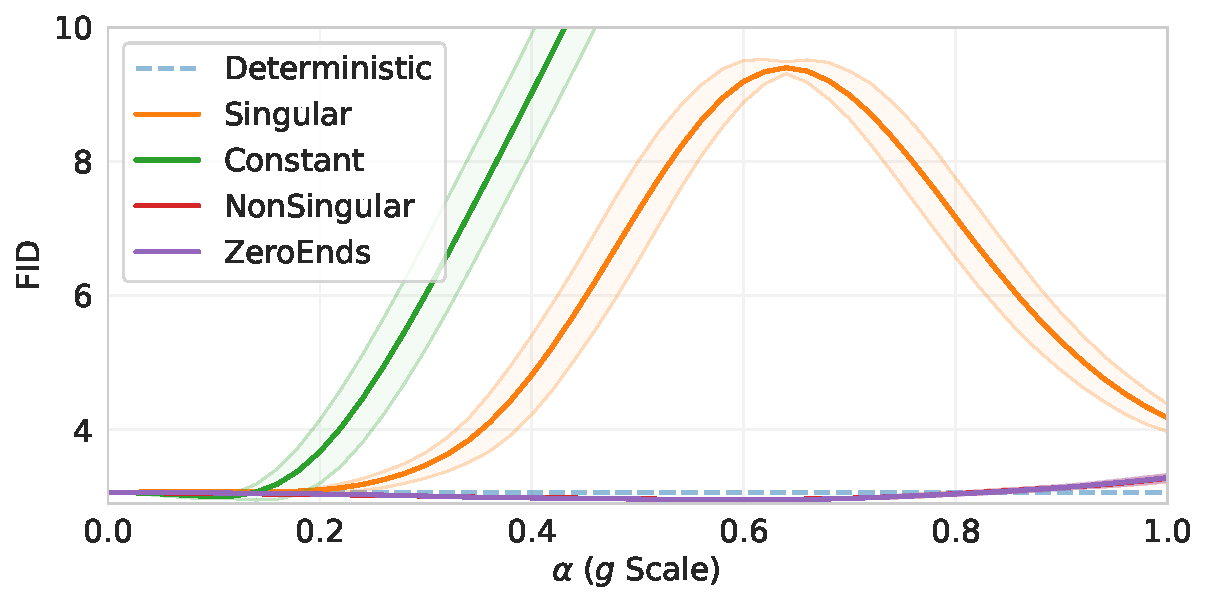
\includegraphics[width=\textwidth]{figs/sampler_scale_comparison_full_w_64.pdf}
\caption{64 $\times$ 64}
\label{fig:alpha_comparison_64}
\end{subfigure}
\begin{subfigure}[b]{0.48\linewidth}
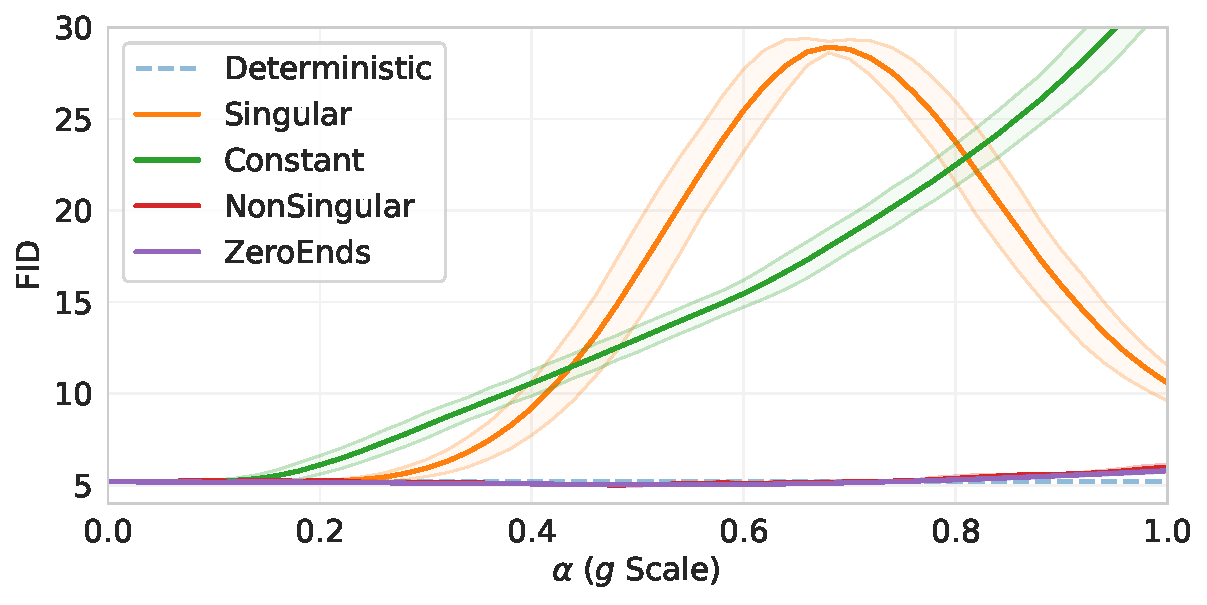
\includegraphics[width=\textwidth]{figs/sampler_scale_comparison_full_w_128.pdf}
\caption{128 $\times$ 128}
\label{fig:alpha_comparison_128}
\end{subfigure}
\caption{%
    \textbf{Non-singular samplers work well over a broad range of $\alpha$.}
    The same plots as \cref{fig:imagenet_fid_alpha}, but showing a larger range of FIDs.
    Note that the Singular sampler is highly non-monotonic as a function of $\alpha$.
}
\label{fig:imagenet_fid_alpha_uncropped}
\end{figure}


\subsection{FID vs $\alpha$}

In \cref{fig:imagenet_fid_alpha_uncropped} we show a larger range FID for various samplers compared in \cref{fig:imagenet_fid_alpha}.
We observe that the Singular sampler tends to perform well only at low scales with an intriguing behavior for higher scales where the FID starts to improve again after worsening significantly.

%%%%%%%%%%%%%%%%%%%%%%%%%%%%%%%%%%%%%%%%%%%%%%%%%%%%%%%%%%5
\subsection{Effect of diffusion coefficient magnitude on samples}
\label{sec:diff_coeff_mag_qual}

We qualitatively visualize the effect of diffusion coefficient magnitude for the three SDEs discussed in the main paper.
\cref{fig:constantg_scale} visualizes samples for the constant diffusion term SDE as a function increasing coefficient magnitude.
Each column is a different sample starting with the same random draw from $p_1(x_1)$.
Each row corresponds to a different magnitude for the diffusion coefficient $g(t)$.
\cref{fig:nonsingular_scale,fig:singular_scale} visualize samples with a similar scheme for the non-singular and singular SDE.

\subsection{Classifier-free guidance samples}
\cref{fig:qual_alpha_vs_lambda} shows additional samples using classifier-free guidance with NonSingular at different values of $\alpha$ and $\lambda$, as in \cref{fig:imagenet_cfg}.

\begin{figure}[tbp]
\small
\caption{NonSingular Sampler written in JAX.}
\label{lst:nonsingular_code}
\begin{lstlisting}[language=Python]
def non_singular_sampler(
    rng, num_samples, model, params, labels, g_scale, num_steps=1000,
    batch_size=10, image_size=64, num_channels=3, num_classes=1000,
    n=1, m=0):
  """Draw samples from the model."""
  p_1_samples = []
  p_0_samples = []
  t = jnp.linspace(1., 0., num_steps+1)
  t_ones = jnp.ones([batch_size, 1, 1])

  # Sampler loop body
  def body_fn(i, z):
    z, labels, rng = z
    tb = t[i] * t_ones
    z_hat = model.apply({'params': params}, z, (1 - tb), labels)
    v = -z_hat
    b = g_scale
    g = b * jnp.power(tb, n / 2) * jnp.power(1 - tb, m / 2)
    s_u = -((1-tb) * v + z)
    fr = (v - jnp.square(b) * jnp.power(tb, n-1
          * jnp.power(1-tb, m) * s_u / 2)
    rng, key = jax.random.split(rng)
    dt = t[i+1] - t[i]
    dbt = (jnp.sqrt(jnp.abs(dt))
           * jax.random.normal(key, shape=z.shape))
    z = z + fr * dt + g * dbt
    return z, labels, rng

  max_steps = num_samples // batch_size
  for _ in range(max_steps):
    # Sample from p_1
    rng, key = jax.random.split(rng)
    z = sample_from_prior(
      key, shape=[batch_size, image_size, image_size, num_channels])
    p_1_samples.append(z)

    # Run the sampler
    rng, key = jax.random.split(rng)
    init_val = (z, labels, key)
    z, _, _ = jax.lax.fori_loop(
        lower=0, upper=num_steps, body_fun=body_fn, init_val=init_val)
    p_0_samples.append(z)

  p_1_samples = jnp.concatenate(p_1_samples, axis=0)
  p_0_samples = jnp.concatenate(p_0_samples, axis=0)
  return p_1_samples, p_0_samples
\end{lstlisting}
\end{figure}

\begin{figure}
\centering
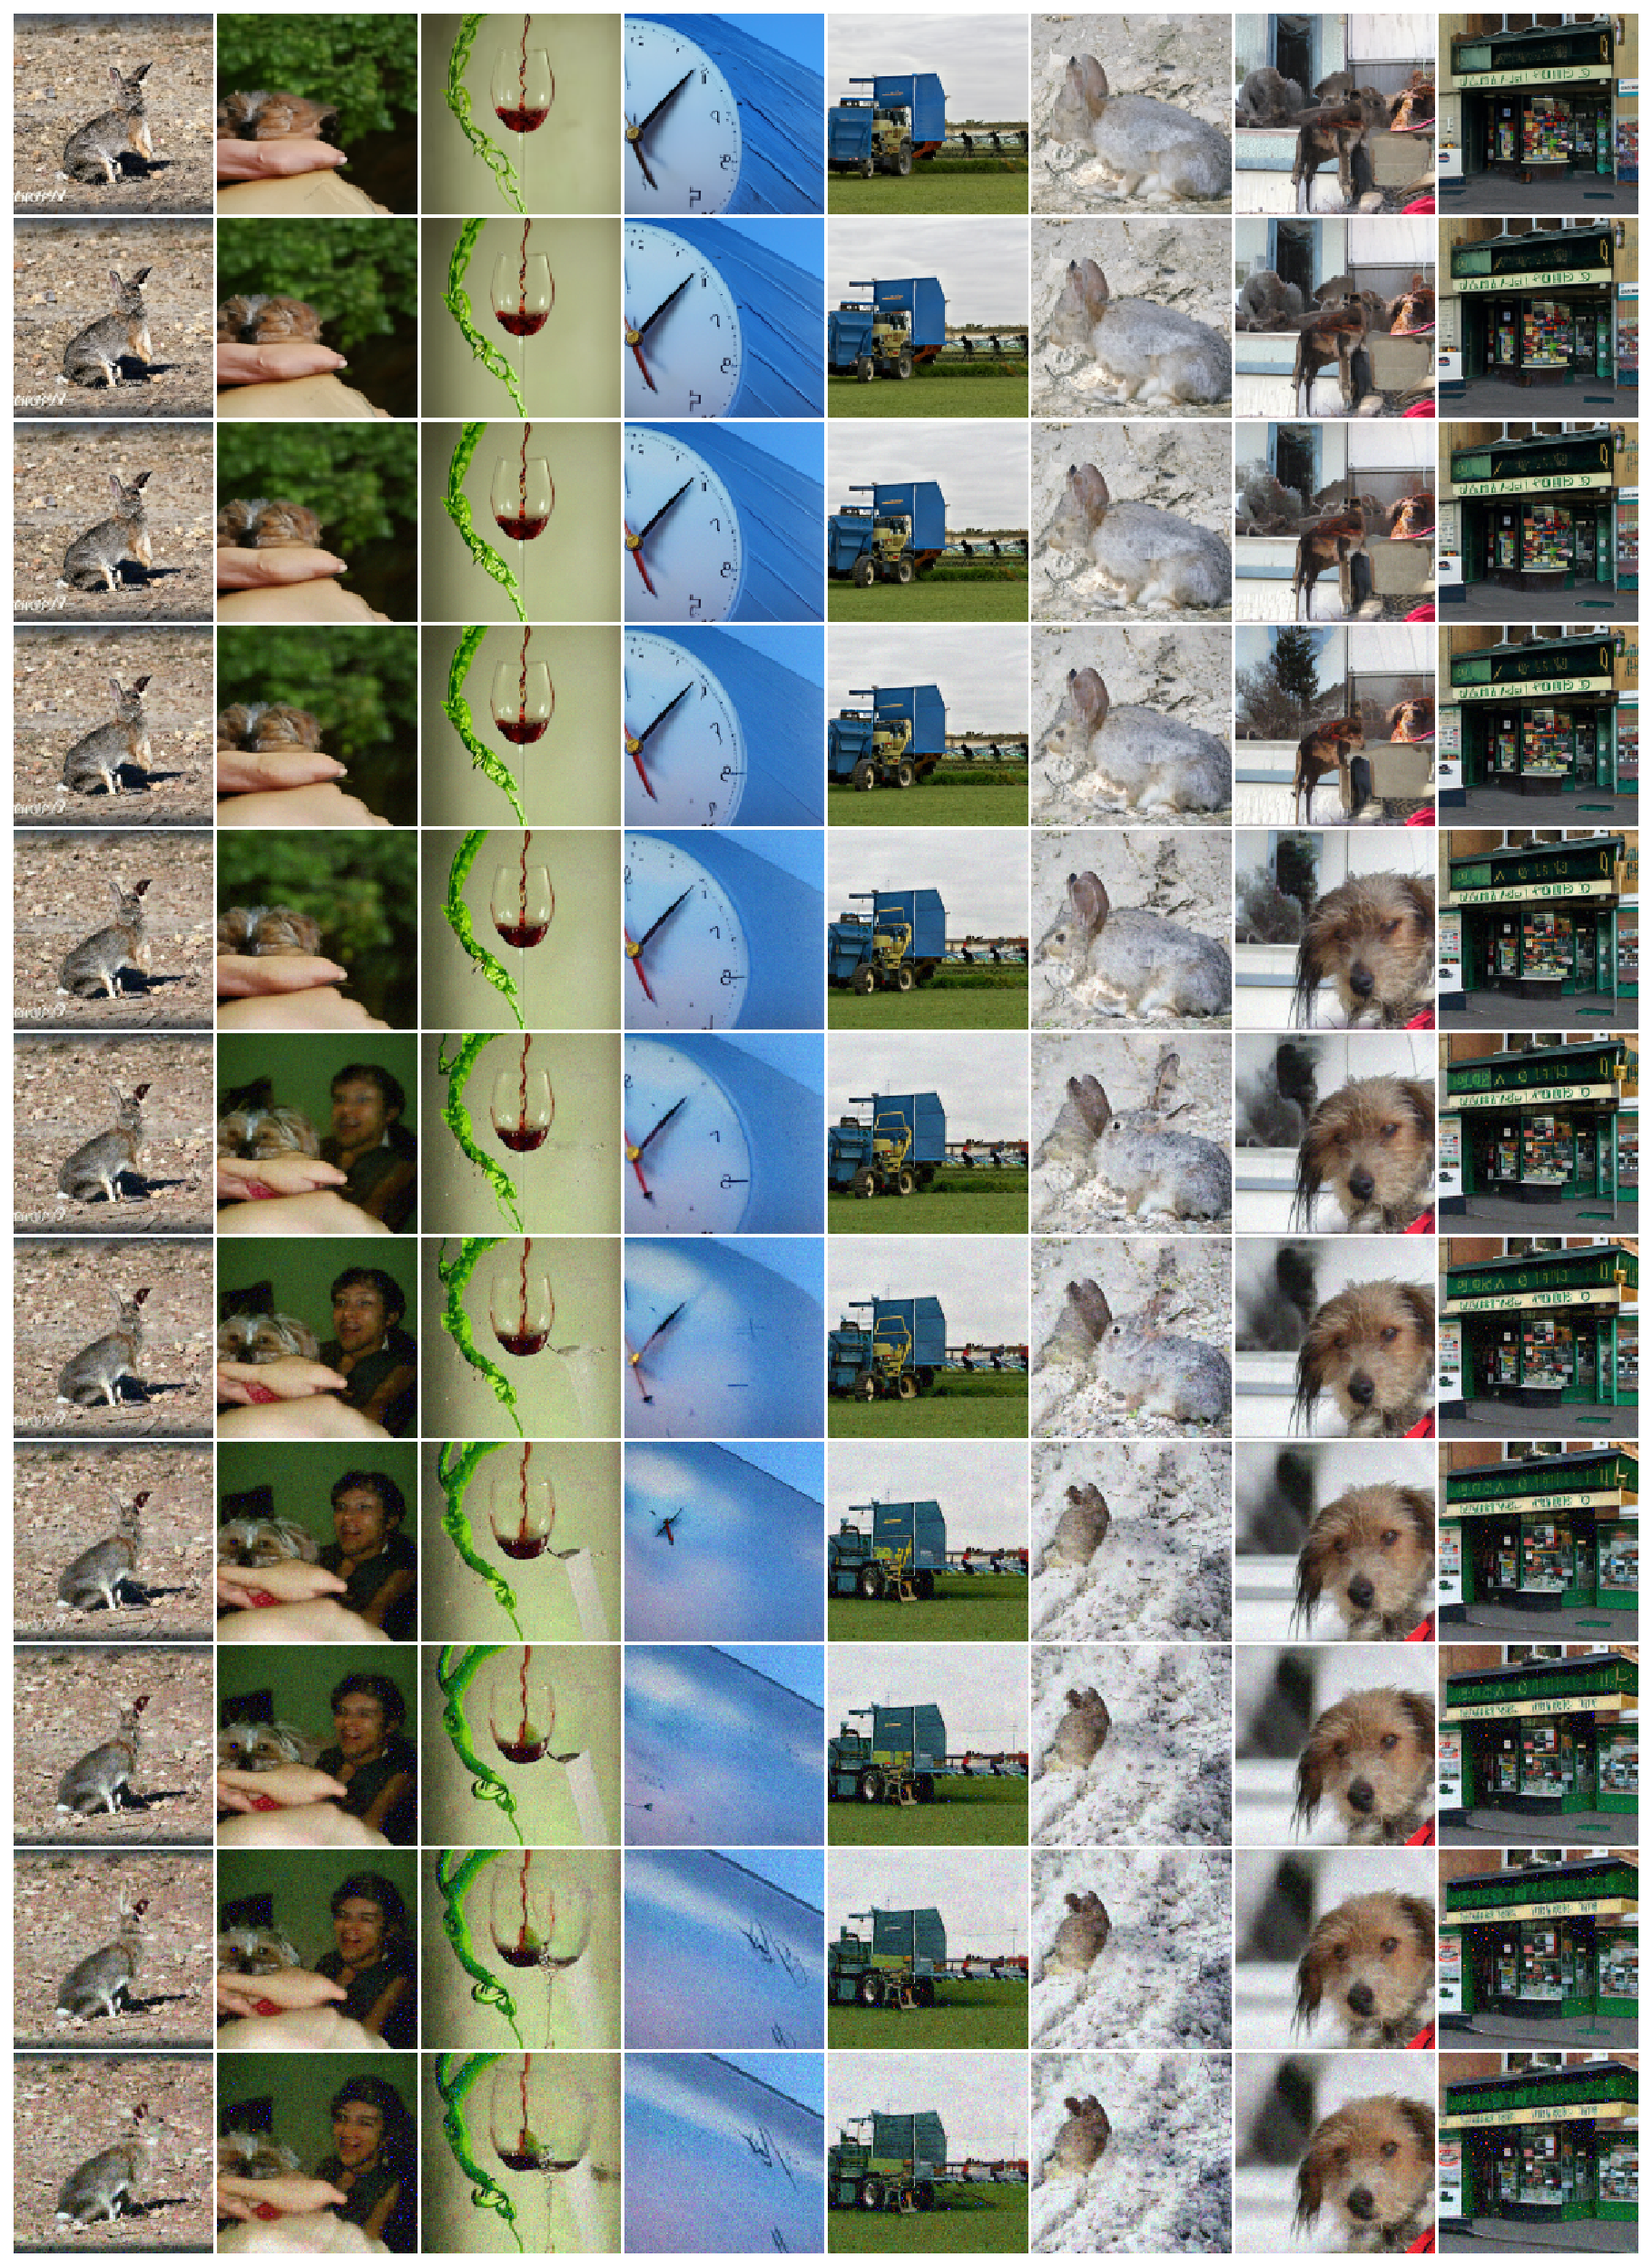
\includegraphics[width=0.95\textwidth]{figs/constantg_noise_scale.pdf}
\caption{%
    \textbf{Constant samples with increasing scaling $\alpha$.}
    Each row displays samples at a particular $g$-scale, from $0$ increasing to $1$ in the increments of $0.1$ from top to bottom.
    Sampling for each columns starts off with the same initial noise image and conditioning class.
}
\label{fig:constantg_scale}
\end{figure}

\begin{figure}
\centering
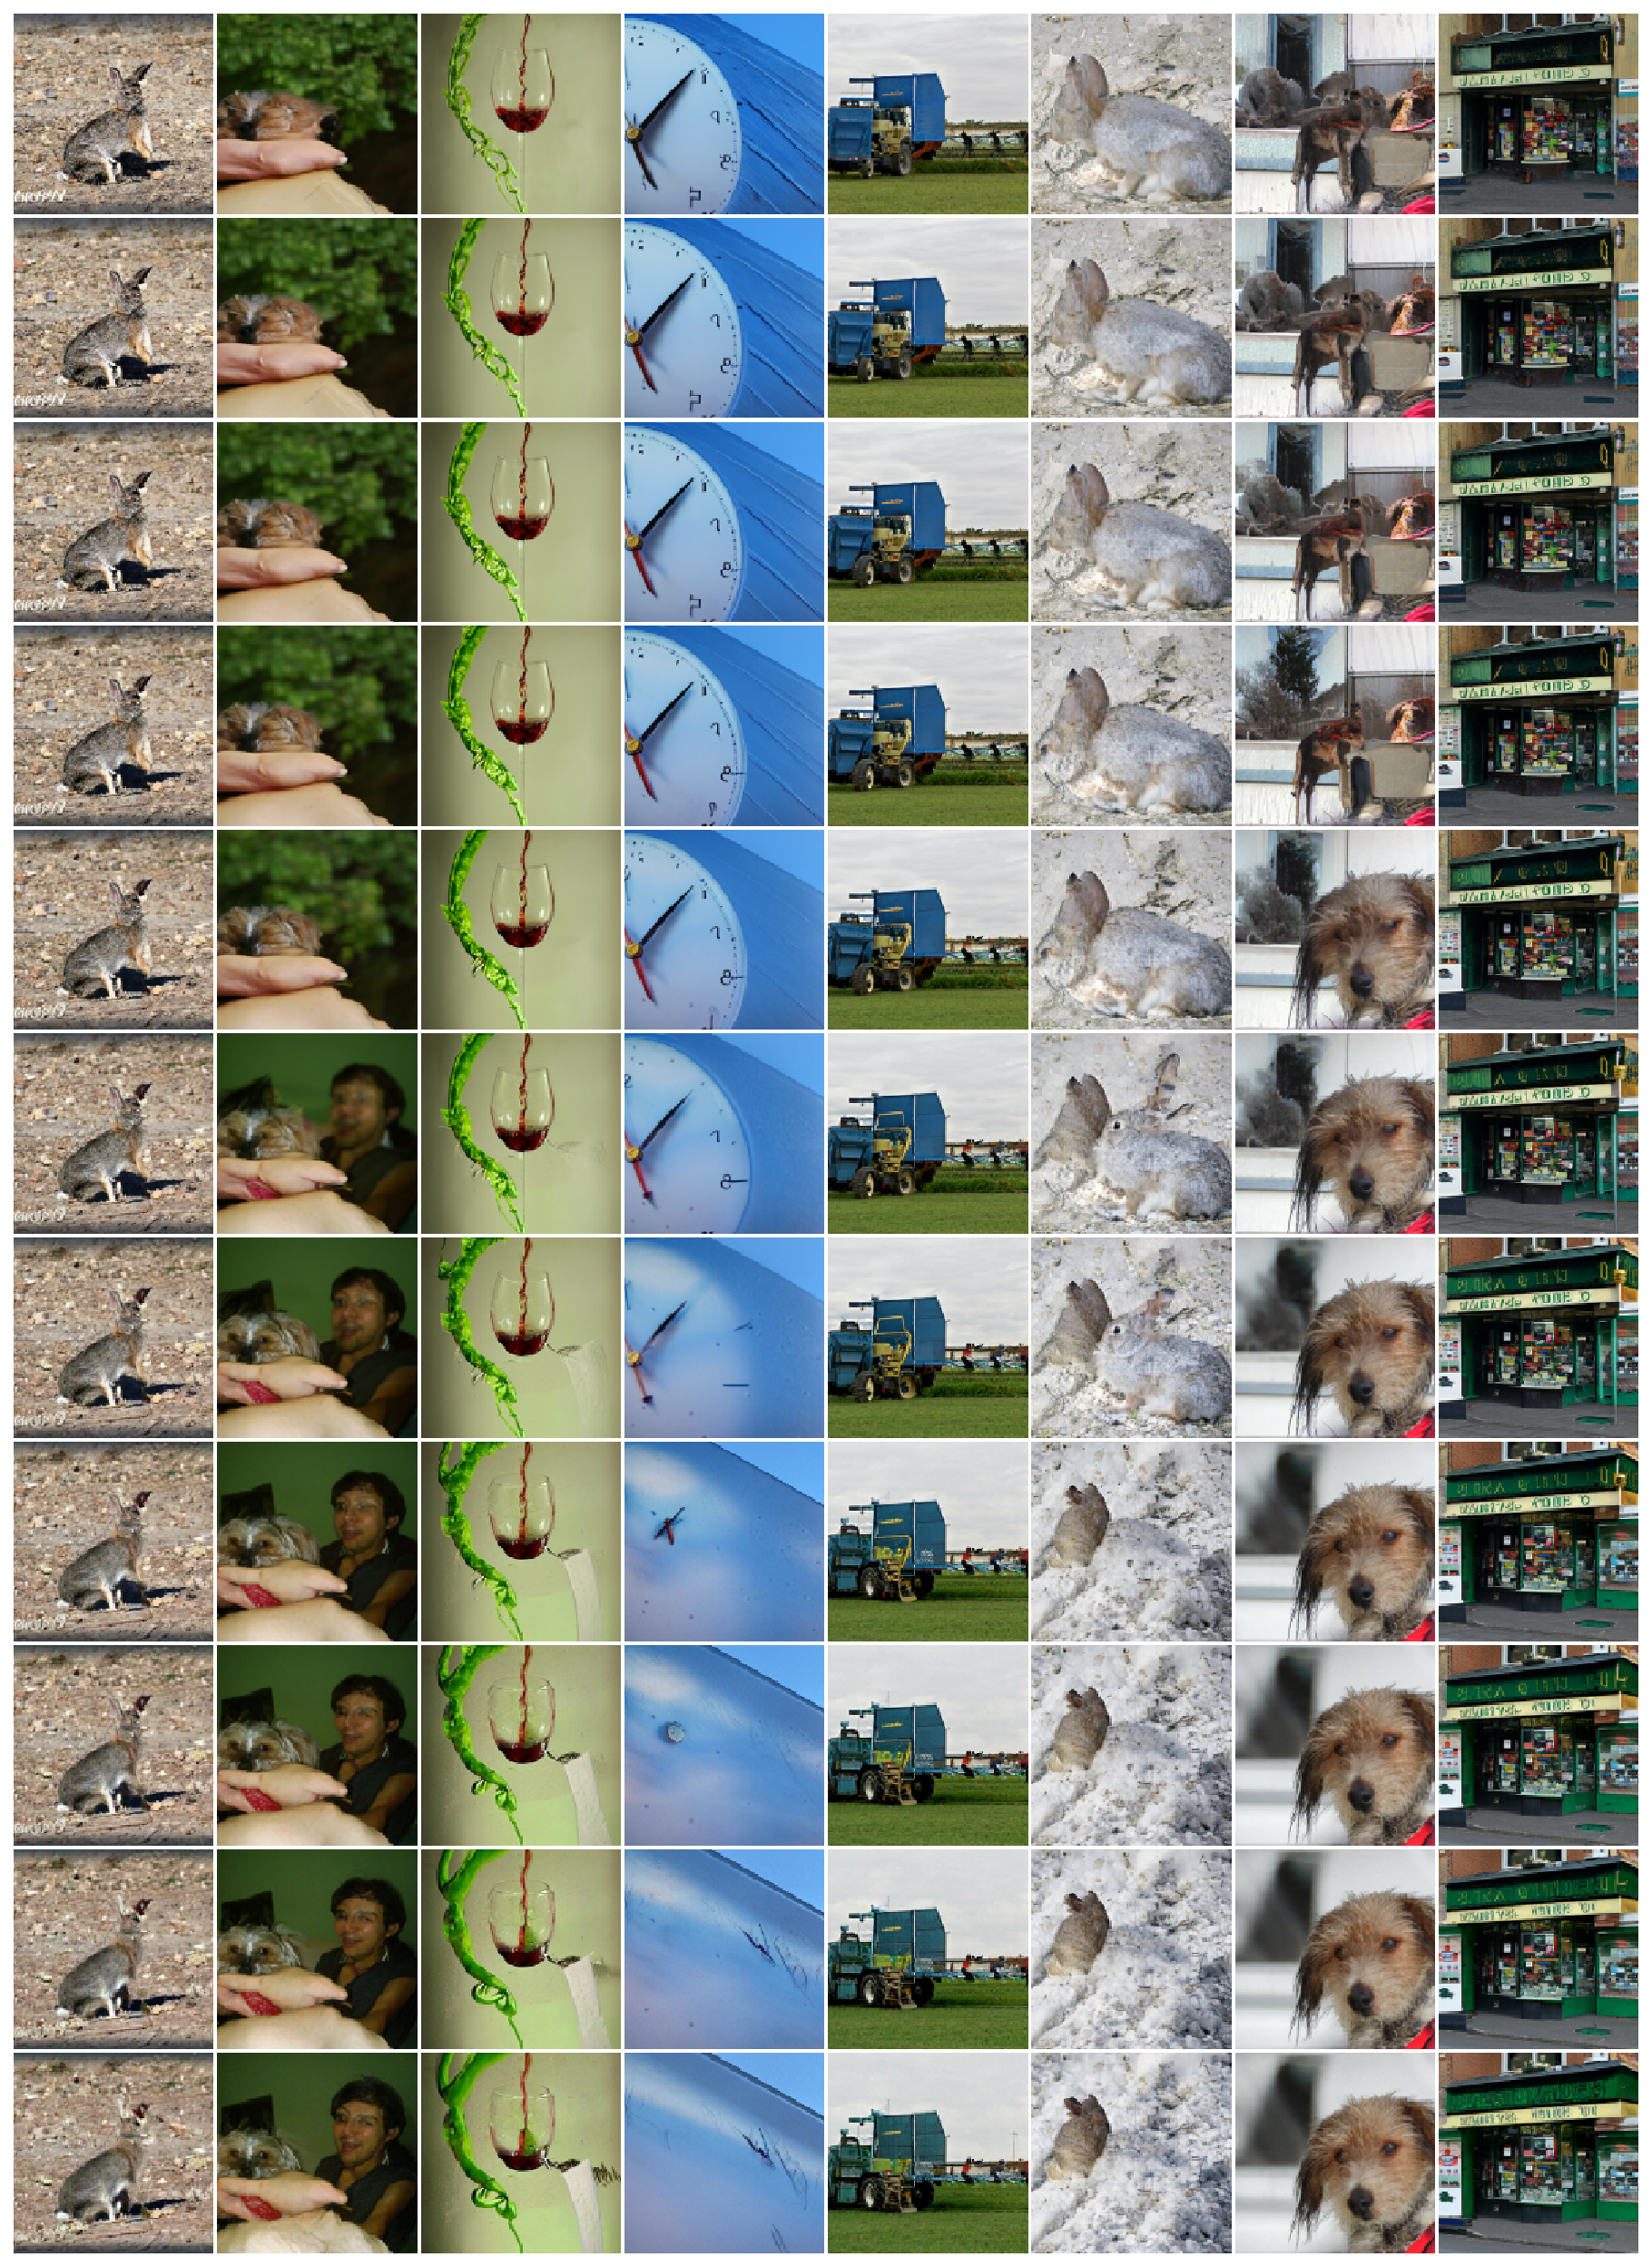
\includegraphics[width=0.95\textwidth]{figs/nonsingular_noise_scale.pdf}
\caption{%
    \textbf{NonSingular samples with increasing scaling $\alpha$.}
    Each row displays samples at a particular $g$-scale, from $0$ increasing to $1$ in the increments of $0.1$ from top to bottom.
    Sampling for each columns starts off with the same initial noise image and conditioning class.
}
\label{fig:nonsingular_scale}
\end{figure}

\begin{figure}
\centering
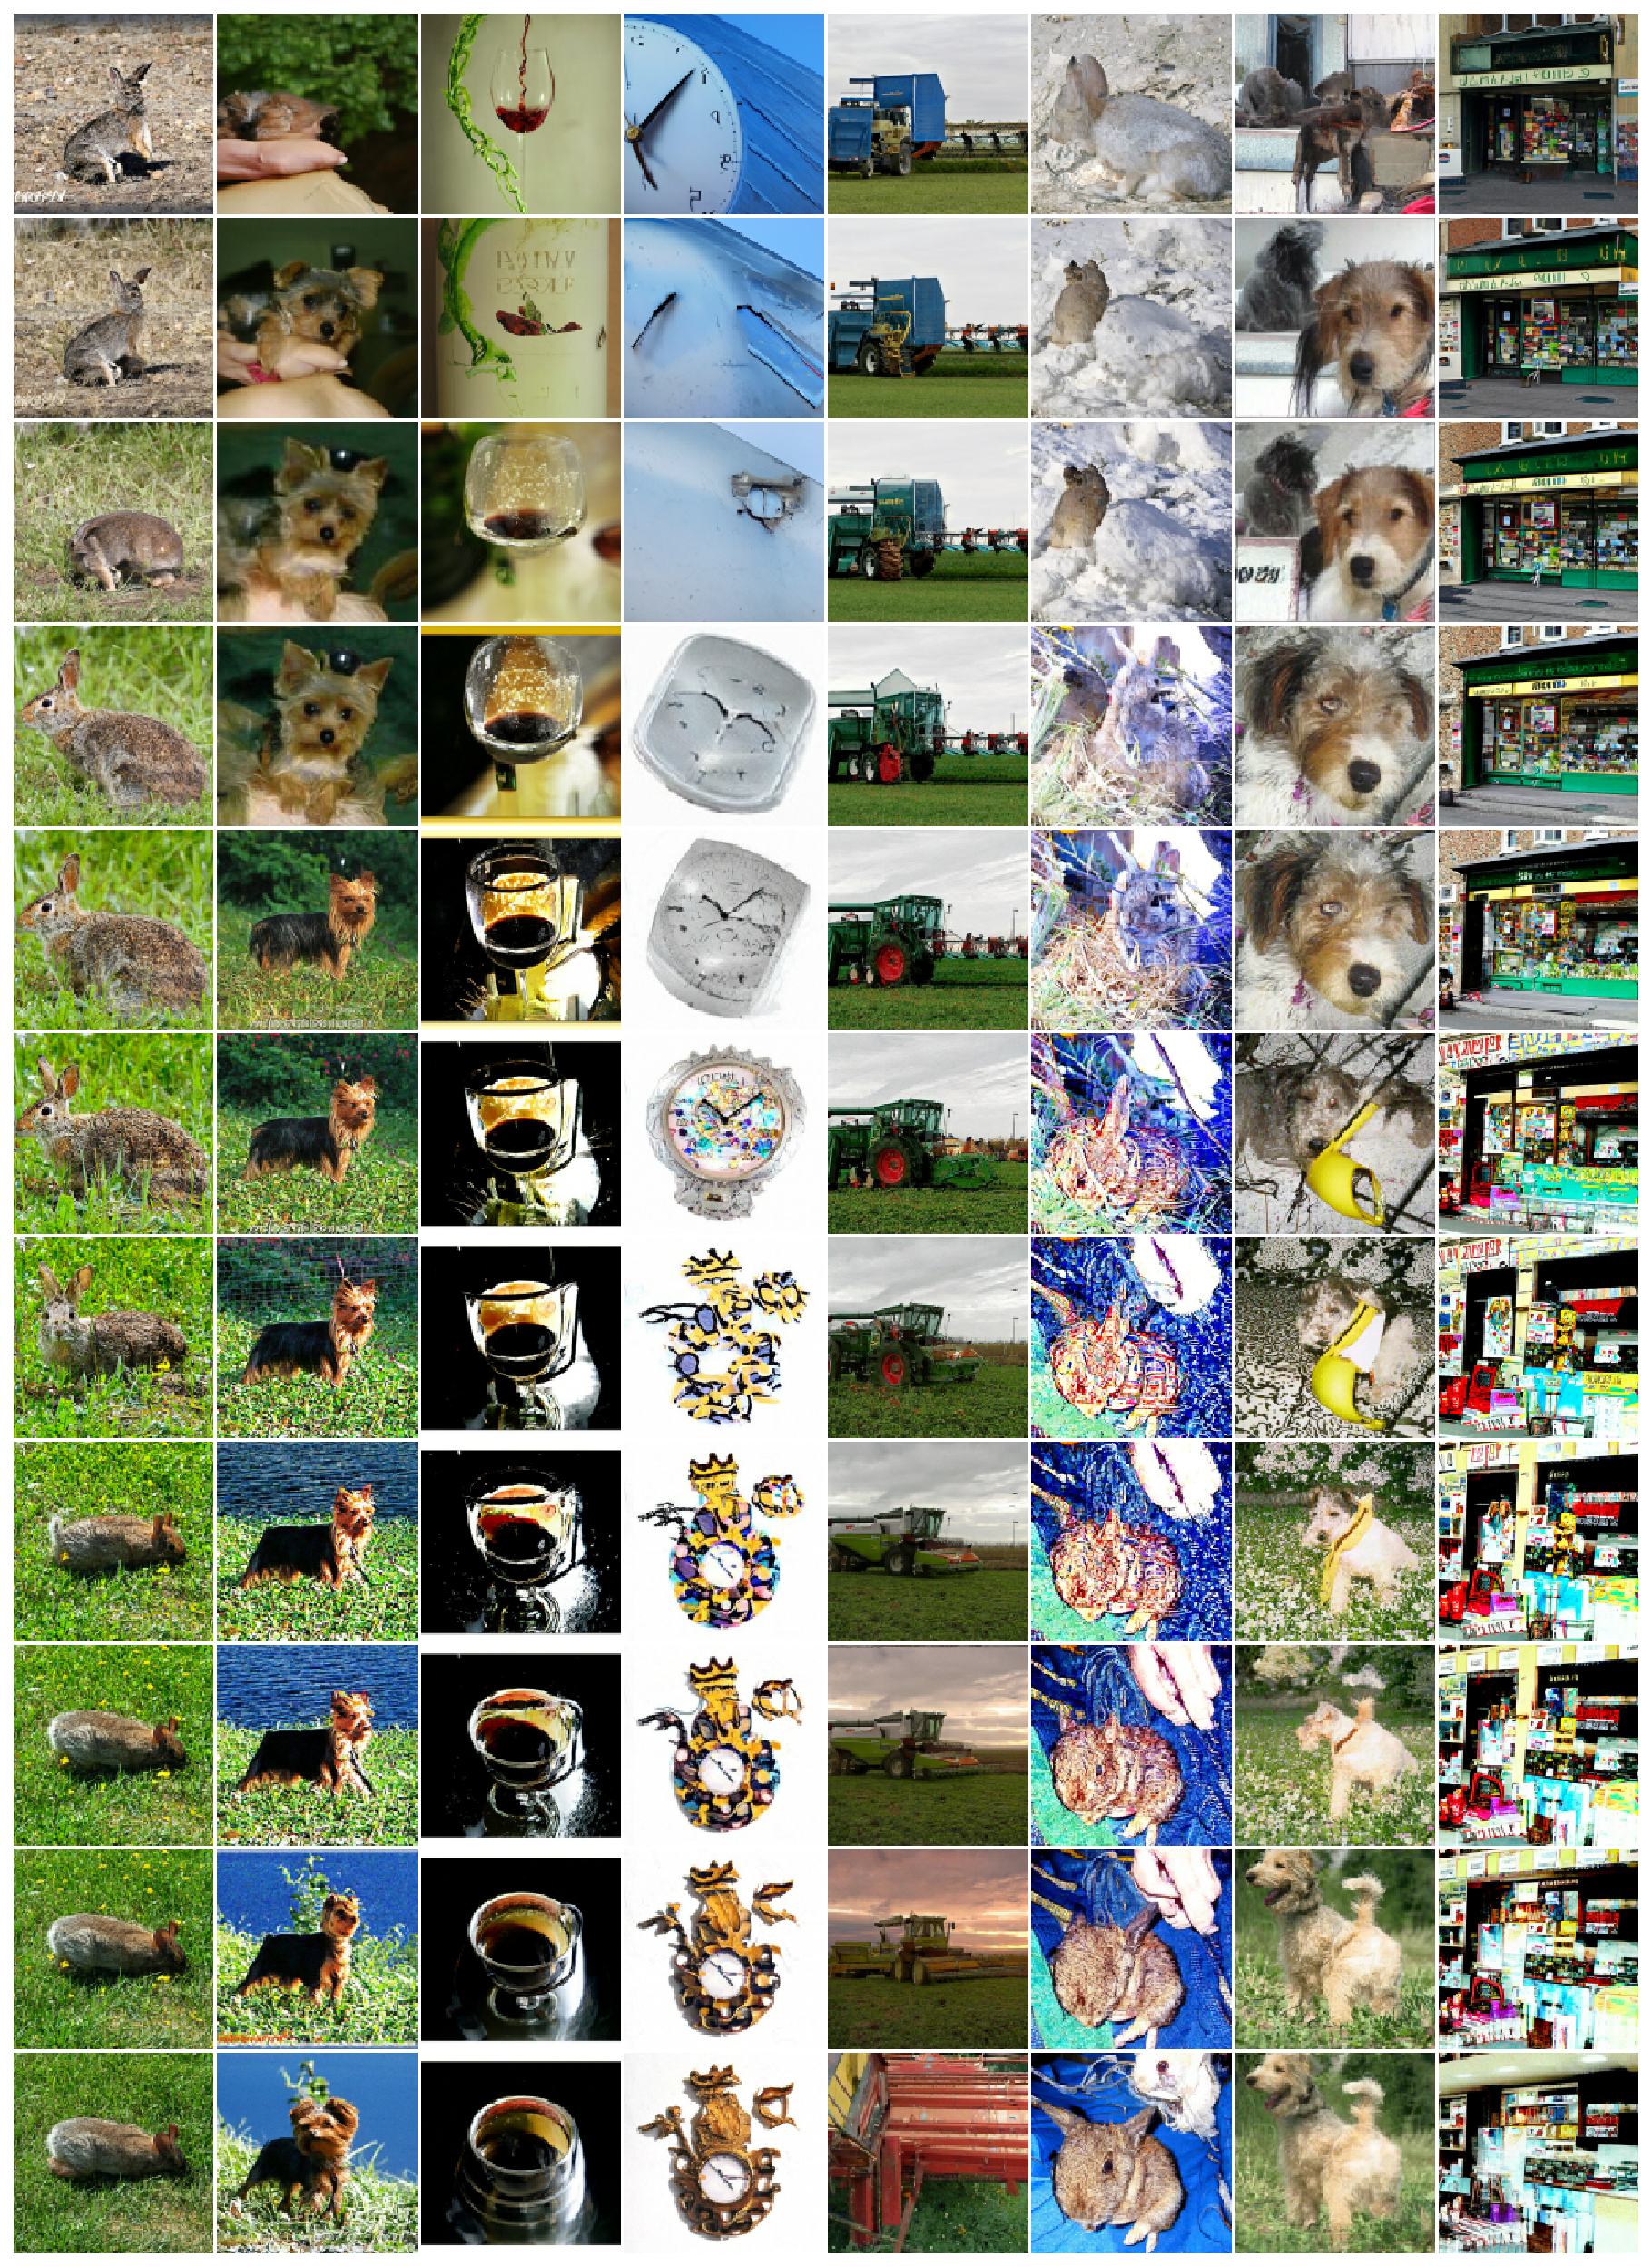
\includegraphics[width=0.95\textwidth]{figs/singular_noise_scale.pdf}
\caption{%
    \textbf{Singular samples with increasing scaling $\alpha$.}
    Each row displays samples at a particular $g$-scale, from $0$ increasing to $1$ in the increments of $0.1$ from top to bottom.
    Sampling for each columns starts off with the same initial noise image and conditioning class.
}
\label{fig:singular_scale}
\end{figure}

\begin{figure}
\centering
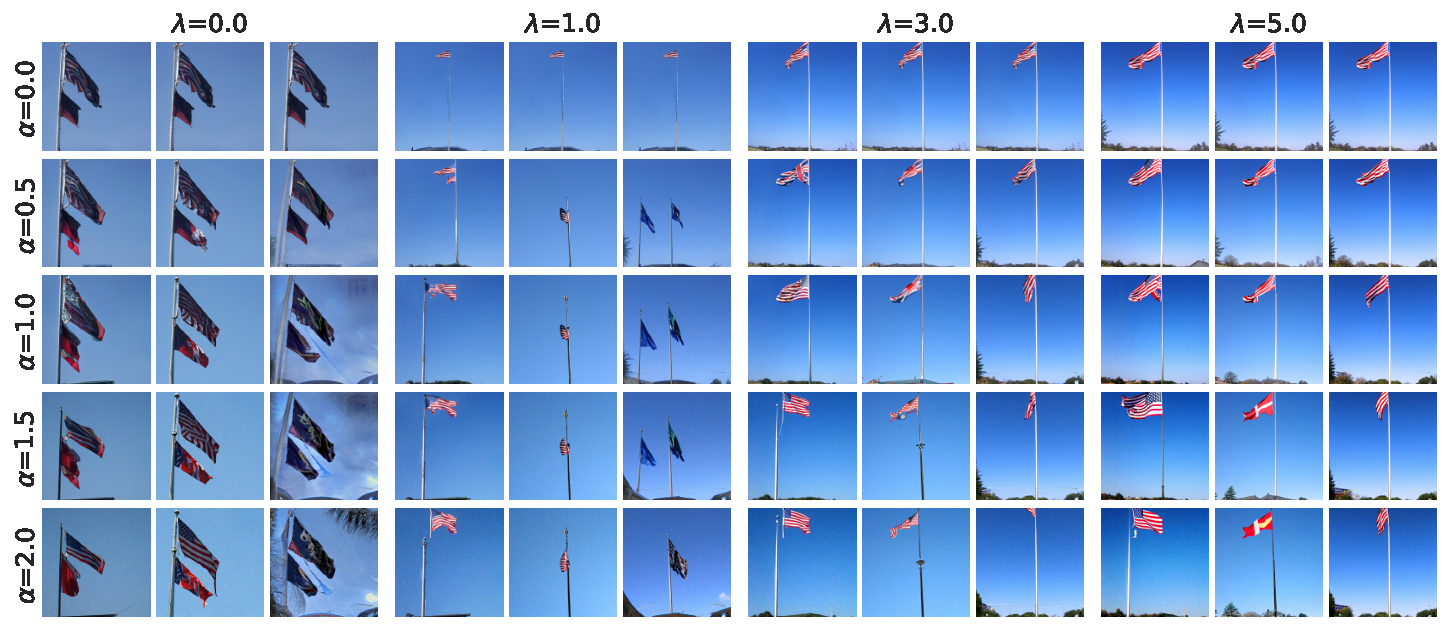
\includegraphics[width=0.99\textwidth]{figs/gscale_vs_cfg_im_6.pdf}
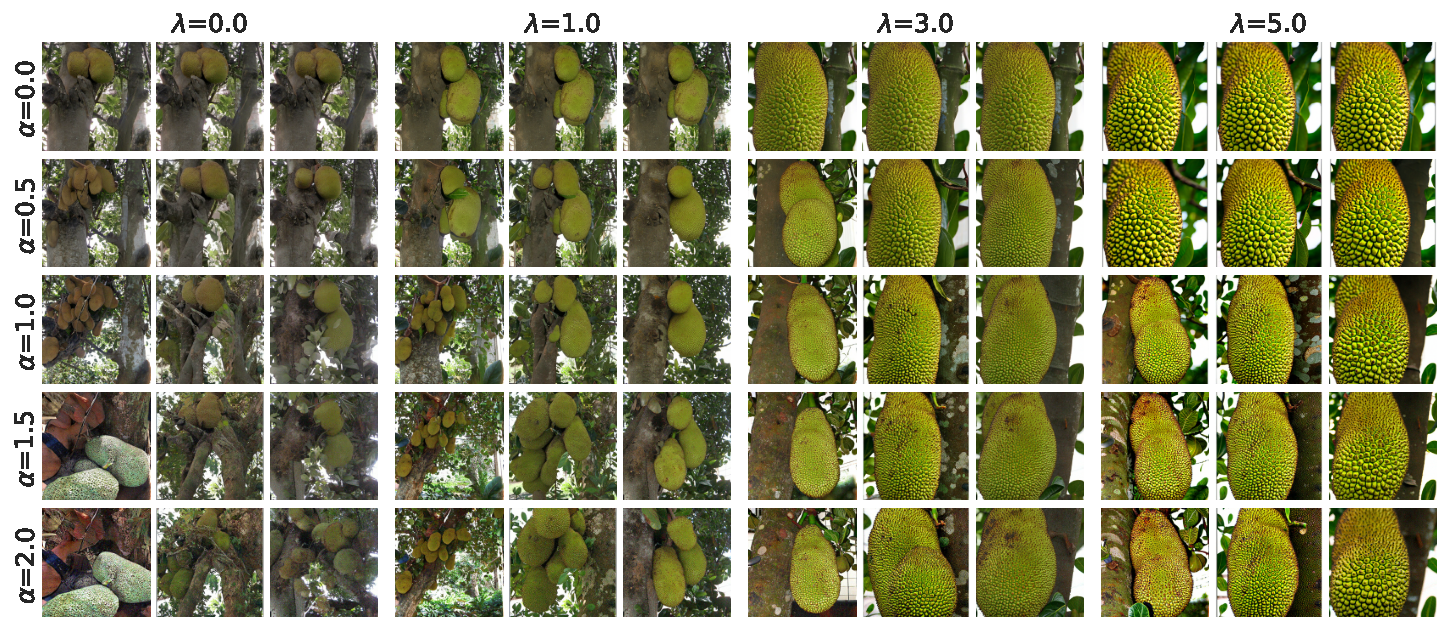
\includegraphics[width=0.99\textwidth]{figs/gscale_vs_cfg_im_1.pdf}
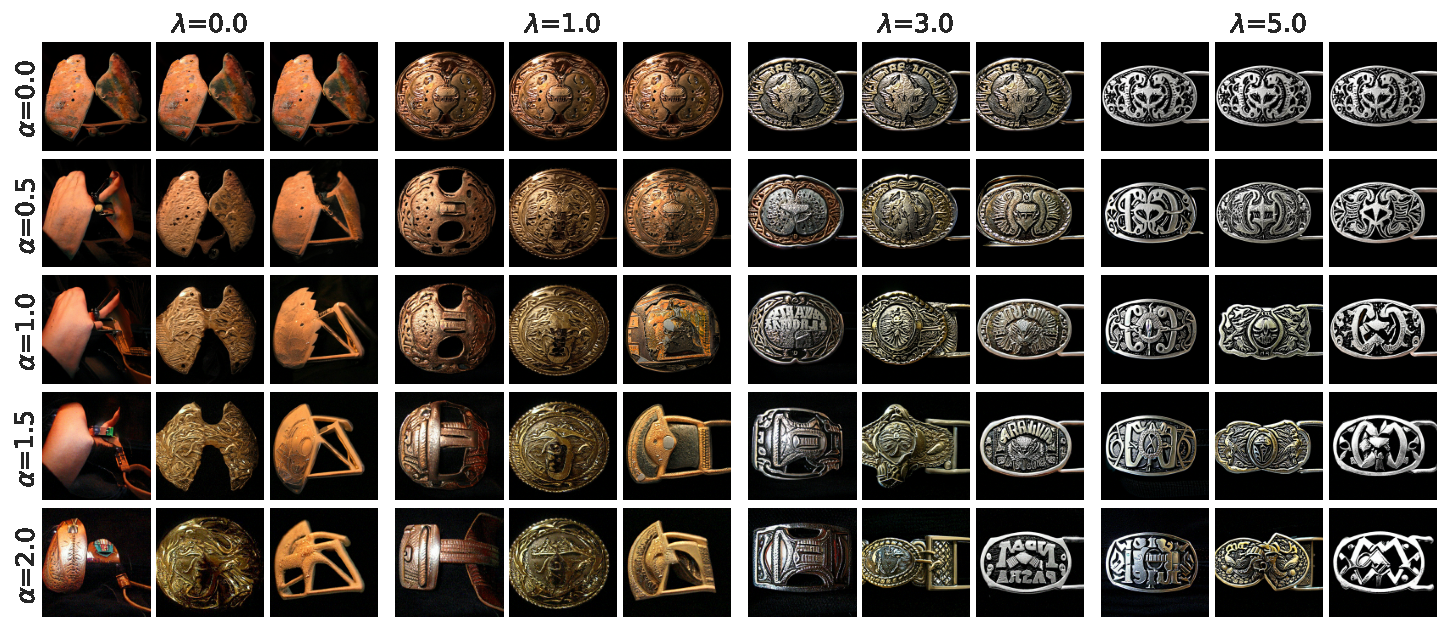
\includegraphics[width=0.99\textwidth]{figs/gscale_vs_cfg_im_2.pdf}
\caption{%
    \textbf{Stochastic sampling improves diversity at all classifier-free guidance levels.}
    Additional results as in \cref{fig:imagenet_cfg}, described in \cref{sec:imagenet_experiments}.
}
\label{fig:qual_alpha_vs_lambda}
\end{figure}

